\chapter{Fundamentals of magnetophoresis and its simulation}\label{ch:chapter2_theory}

%\textit{Microfluidic devices for manipulating fluids are widespread and finding uses in many scientific and industrial contexts nowadays. Applications are reaching from chemical, biological or even optical and information industry. Their design often requires unusual geometries and the interplay of multiple physical effects. Even as the basic science and technological demonstrations develop, other problems must be address to complete the cycle of development. The solutions to these problems will require imagination and ingenuity.}

%\textit{The key item in this work is the “switchable” magnetic (i.e., superparamagnetic) particle. Magnetophysical principles presented in the following chapters are directly related to the magnetic properties and separation behaviour of the engineered particles. Although their magnetic separation can easily be demonstrated, the theory behind the observable process is important for the control of the particle separability.}

\section{Introduction}
In this chapter the fundamentals of microfluidics and magnetism, the two main fields involved in magnetophoresis, will be explained and their basic mathematical models will be derived.\ Additionally, the numerical methods to simulate the magnetic field using FEM are shown.\\
This chapter is by no means exhaustive.\ Further details on fluid dynamics and magnetism, as well as finite element methods, can be found in many published textbooks (e.g.~\cite{White2006,Happel2012,Brenner2008,Cheng2012}).\
%
\section{Fluid motion in microfluidic systems}\label{sec:fluidMotionInMicrofluidicSystems}
In general, the flow field inside a fluid channel can be described by the incompressible Navier-Stokes equations, which represent the conservation of momentum (Equation~\ref{eqn:navierStokesEquation}) and conservation of mass (Equation~\ref{eqn:continuityEquation})~\cite{Happel2012}:\
\begin{eqnarray}
	\rho_{f} \left( \frac{\partial\mathbf{u}}{\partial t} + (\mathbf{u}\cdot\nabla)\mathbf{u} \right) &=& -\nabla p + \eta_{f} \nabla^{2}\mathbf{u}  	
	\label{eqn:navierStokesEquation} \\
	\nabla \cdot \mathbf{u}&=& 0
	\label{eqn:continuityEquation}
\end{eqnarray}
where $\mathbf{u}$, $\rho_{f}$, $\eta_{f}$ and $\nabla p$ are the velocity vector, the fluid density, fluid dynamic viscosity and pressure gradient, respectively.\ Equation~\ref{eqn:navierStokesEquation} assumes the fluid to be incompressible and isotropic (Newtonian fluid), which means the fluid's density $\rho_f$ as well as its viscosity $\eta_{f}$ can be approximated as constant.\ The different terms in Equation~\ref{eqn:navierStokesEquation} correspond to the inertial forces, the convection force, pressure forces and diffusion forces applied to the fluid.\\
The steady-state continuity equation for an incompressible flow (Equation~\ref{eqn:continuityEquation}) reflects the fact that mass is conserved.\ It states that the rate at which mass enters a system is equal to the rate at which mass leaves the system.\\
To completely characterise the flow field described by the Navier-Stokes equations (Equation~\ref{eqn:navierStokesEquation} and Equation~\ref{eqn:continuityEquation}), also a set of boundary conditions is needed. The boundary conditions need to include the pressure difference on the in- and outlets of the domain as well as the velocities of the bounding surfaces (if these are moving in the frame of reference).\ In this work, the geometry is assumed to be a rectangular duct with no moving side walls and a \textit{no-slip} condition (Dirichlet boundary condition) with the fluid velocity specified at the inlets and pressure prescribed at the outlets:\
\begin{eqnarray}
	\mathbf{u} = 0 && \text{on $\Gamma$}
	\label{eqn:dirichletBoundaryCondition}
\end{eqnarray}
where $\Gamma$ represents the boundaries of the domain, i.e. the channel's side walls.\ The velocity at the different inlets is assumed to be uniform across the entire area but will be varied in its magnitude.\
%
\subsection{Steady unidirectional flow in a rectangular duct}\label{sub:steadyUnidirectionalFlowInRectangularDuct}
On the micro-scale, laminar flow is typically achieved~\cite{Whitesides2006}.\ Whether a flow regime is laminar or turbulent can be determined by calculating the dimensionless Reynolds number, which represents the ratio of inertial force to viscous force~\cite{White2006}:\
\begin{equation}
	\text{Re} = \frac{\rho_{f}u_{f}D_{H}}{\eta_{f}}
 	\label{eqn:reynoldsNumber}
\end{equation}
Here, $u_{f}$ is the fluid velocity (in one direction) and $D_{H}$ is the hydraulic diameter (characteristic length) of the fluid channel.\ For a rectangular duct, the hydraulic diameter, $D_{H}$ is given by the ratio between the cross section and the wetted area~\cite{GaryLeal1993}:\
\begin{equation}
 	D_{H} = \frac{4A}{W}
 	\label{eqn:hydraulicDiameter}
\end{equation}
with the cross sectional area $A$ and the wetted perimeter $W$ of the cross section.\ For a rectangular cross section, $A$ and $W$ can be described as~\cite{GaryLeal1993}:\
\begin{eqnarray}
	A = w_{0}h_{0} \\
	W = 2(w_{0}+h_{0})
\end{eqnarray} 
where $w_{0}$ and $h_{0}$ are the width and the height of the rectangular fluid channel.\ In this work the hydraulic diameter is $D_{H} \approx 0.7$ mm.\\
Going from a turbulent to a laminar regime, or vice versa, does not occur abruptly but is a continuous transformation process without a clear transition point.\ In the literature, a transition threshold of $\text{Re} \approx 2300$ is normally given as a rule of thumb~\cite{Happel2012}.\\
In most circumstances in microfluidics, the Reynolds number is around unity or even one order of magnitude smaller, ruling out turbulent flows in the channel (here, $1.4 \leq \text{Re} \leq 3.7$).\ At low Reynolds numbers the flow is dominated by viscous drag rather than inertial forces, and is characterized by a continuous and ordered fluid motion in contrast to turbulent flow which is irregular.~\cite{Purcell1977}.\ For these conditions the entrance length is defined as the distance between the inlets and the point that the flow becomes fully developed (time invariant or steady).\ This distance is directly proportional to the Reynolds number and can be estimated by~\cite{Kays2012}:\
\begin{equation}
	L_{H} \approx 0.06 D_{H} \text{Re}
	\label{eqn:entranceLength}
\end{equation}
The maximum entrance length $L_{H}$ for the highest Reynolds Number used in this thesis is approximately $155$ $\mu$m, which is more than $100$ times smaller, than the channel length of the devices used in this thesis (see Chapter~\ref{ch:experiments}).\\
For a unidirectional flow that is assumed to be steady-state and fully developed, the inertial force ($\partial \mathbf{u}/\partial t$) and the convective terms ($\mathbf{u}\cdot\nabla\mathbf{u}$) are all equal to zero and thus, can be omitted.\ Without the nonlinear convection and time dependence, the Navier-Stokes equation (Equation~\ref{eqn:navierStokesEquation}) can be simplified.\ The resulting linear equations governing the velocity distribution in the fluid are~\cite{Happel2012}:\
\begin{equation}
	\eta_{f} \nabla^{2}\mathbf{u} = \nabla p 
	\label{eqn:stokesEquation}
\end{equation}
Equation~\ref{eqn:stokesEquation} together with the continuity equation (Equation~\ref{eqn:continuityEquation}) are known as the Stokes equations.\ An analytical solution to Equation~\ref{eqn:stokesEquation} using the Dirichlet boundary conditions given in Equation~\ref{eqn:dirichletBoundaryCondition} can be found for a number of simple geometries.\ In the absence of moving beads in the fluid, the hydrodynamics of a rectangular microfluidic channel in the limit of laminar flow is standard textbook material.\ The solution to Equation~\ref{eqn:stokesEquation} gives the so called Poiseuille flow for a channel of rectangular cross section and can be mathematically expressed by the following infinite Fourier series summation~\cite{White2006}:\
\begin{equation}
	u_{f}(x,y) = \frac{4h_{0}^{2}}{\eta_{f}\pi^3}\left(-\frac{dp}{dz}\right)\sum_{k=0}^{\infty}(-1)^{k}\times\left\{ 1 - \frac{\cosh\Big[\frac{(2k+1)\pi x}{h_{0}}\Big]}{\cosh\Big[\frac{(2k+1)\pi w_{0}}{2h_{0}}\Big]} \right\} \frac{\cos\Big[\frac{(2k+1)\pi y}{h_{0}}\Big]}{(2k+1)^{3}}
	\label{eqn:velocityProfileRectangularDuct}
\end{equation}
where $h_{0}$ and $w_{0}$ are the height and the width of the fluid channel and $dp/dz$ describes the pressure drop along $z$.\ The pressure driven velocity profile across a cross section of a rectangular microchannel is shown in Figure~\ref{fig:velocityProfile3D}.\
\begin{figure}[htb]
	\centering
   \includegraphics[width=0.6\textwidth]{img/chapters/chapter_2_theory/3DvelocityProfileMesh_final.png}
	\caption[Schematic of a 3D velocity profile of a unidirectional flow in a rectangular duct of a viscous fluid]{Schematic of a 3D velocity profile of a unidirectional flow in a rectangular duct of a viscous fluid. In this analytical calculation the width ($w_{0}$) and the height ($h_{0}$) of the channel is set to $500$ $\mu$m and the fluid channel's length ($l_{0}$) is set to $10$ mm.}
\label{fig:velocityProfile3D}
\end{figure}
%
\subsubsection{Hydraulic resistance in microfluidic systems}
\label{subsec:hydraulicResistanceInMicrofluidicSystems}
In Section~\ref{sub:steadyUnidirectionalFlowInRectangularDuct} the pressure-driven, steady-state flow of an incompressible Newtonian fluid through a straight channel is studied.\ It is found that a constant pressure drop results in a constant flow rate.\ This result can be summarised in the Hagen-Poiseuille law~\cite{Bruus2007}:\
\begin{equation}
	\Delta p = R_{H}\dot{Q} 
	\label{eqn:hagenPoiseuille}
\end{equation}
where $\Delta p$ is the pressure drop along the channel, $\dot{Q}$ the resulting flow rate through the channel and $R_{H}$ a proportionality factor known as the hydraulic resistance.\ The hydraulic resistance is due to viscous dissipation of mechanical energy into heat by internal friction in the fluid.\ For a straight and rigid channel of length $l_{0}$ and rectangular cross-section ($w_{0} \times h_{0}$), the hydraulic resistance can be approximated as~\cite{Bruus2007}:\
\begin{equation}
	R_{H} \approx \frac{12\eta_{f}l_{0}}{h_{0}^{3}w_{0}\left[1-0.63(h_{0}/w_{0})\right]}
	\label{eqn:hydraulicResistance}
\end{equation}
Equation~\ref{eqn:hydraulicResistance} assumes that the fluidic channel is perfectly straight and that its cross section is not changing along its length, which is true for all the microfluidic systems analysed in this work.\\
Typically, the fluid flow is subject to a no-slip boundary condition at the walls and thus the actual hydraulic resistance will depend on the perimeter as well as the cross-section area.\ With the miniaturization of microfluidic systems, their surface area to volume ratio increases.\ This leads to a high hydraulic resistance and thus results in a high back pressure when liquids are pumped through the system.\ This high back pressure can cause difficulties in the introduction of fluids in microfluidic systems and therefore, should be taken into consideration when microfluidic channels in LOC systems are designed~\cite{Bruus2007}.\
%
\subsection{Particle laden flow in microfluidic systems}\label{subsec:particleLadenFlowInMicrofluidicSystems}
Particle laden flows refer to a multiphase flow in which one of the phases is continuously connected and the other phase is made up of small, immiscible, and typically dilute particles.\ The above discussion on fluid motion in microfluidic systems does not take a discrete phase into account.\ When particles are added to the flow, they will alter the fluid properties and it is necessary to determine if this effect is significant.\\
Depending on the volume fraction of the dispersed phase, the particle laden flow needs to be modelled differently.\ The particle volume fraction, $\upsilon_{p}$, is described by the ratio~\cite{Elghobashi1994}:\
\begin{equation}
	\upsilon_{p} = \frac{V_{tot}}{V_{unit}}
\end{equation}
where $V_{tot}$ is the total volume of the solid phase in the unit volume $V_{unit}$.\ If the concentration of particles is high ($\upsilon_{p}>10^{-3}$), the particle-particle interaction and its effect on the fluid (four-way coupling) must be modelled.\ For intermediate concentrations ($10^{-6} < \upsilon_{p} < 10^{-3}$), particle-particle interaction may be neglected but the particles still have an effect on their surrounding fluid (two-way coupling).\ For low concentrations ($\upsilon_{p} < 10^{-6}$), the fluid flow is not considerably influenced by the particle flow (one-way coupling)~\cite{Hryb2009}.\\
In most microfluidic cases, the particles occur in low concentrations and are very small, hence the dynamics are governed primarily by the continuous phase.\ The behaviour of the particles in a fluid flow can be characterised by the Stokes number, Stk, which is defined as the ratio of the characteristic time of the particles to a characteristic time of the flow~\cite{Happel2012}:\
\begin{equation}
 \text{Stk} = \frac{\tau_{p} u_{f}}{D_{p}}
\end{equation}
where $u_{f}$ is the velocity of the fluid, $D_{p}$ is the hydraulic diameter of the particle and $\tau_{p}$ is the relaxation time of the particle, which is given by~\cite{Happel2012}:
\begin{equation}
	\tau_{p} = \frac{\rho_{p}d_{p}^{2}}{18\eta_{f}}
\end{equation} 
where $\rho_{p}$ and $d_{p}$ are the particle's density and diameter.\\
The Stokes number is a measure of flow tracer fidelity, which means it gives information about how well particles follow the fluid flow.\ For large Stokes numbers (Stk $\gg 1$), particles will detach from the flow and the particle motion is weakly affected by the flow, whereas for small Stokes numbers (Stk $\ll 1$) the particles follow the streamlines closely, which means the particles are in quasi equilibrium with the surrounding flow.\\
In the present work, a dilute concentration ($\upsilon_{p} \leq 10^{-6}$) and a small Stokes number ($\text{Stk} \approx 10^{-3}$) can be assumed.\ Thus, the flow does not depend on the particle dynamics and therefore can be solved in an uncoupled way.\ This allows calculating the particle laden flow according to Equation~\ref{eqn:stokesEquation} and independently from other particle movements (see Section~\ref{subsec:lagrangianParticleTracking}).\
%
\subsection{Hydrodynamic focusing}\label{subsec:hydrodynamicFocusing}
Hydrodynamic focusing is a widely used technique in microfluidics~\cite{Golden2012,Dziubinski2015}.\ It involves the reshaping of a central stream by varying the pressure of the two sheath flows, as schematically shown in Figure~\ref{fig:hydrodynamicFocusingSchematic}.\ This way, one can achieve precise control of the focused sample stream width and position, which is of crucial importance to magnetic particle separation because of the non-uniform nature of the magnetic force.\ Due to the planar nature of most microfluidic devices only two-dimensional hydrodynamic focusing will be considered here.\
\begin{figure}[htb]
\centering
   \includegraphics[width=0.75\textwidth]{img/chapters/chapter_2_theory/hydrodynamicFocusing.pdf}
	\caption[Hydrodynamic focusing schematic in a three inlet fluidic device]{A schematic of the three inlet channel of the microfluidic device displaying hydrodynamic focusing of a sample flow $\dot{Q}_{c}$ by varying the two sheath flows $\dot{Q}_{s1}$ and $\dot{Q}_{s2}$.}%
\label{fig:hydrodynamicFocusingSchematic}%
\end{figure} 
To mathematically express the width of the sample stream the model for hydrodynamic focusing in a rectangular channel by Lee \etal{}~\cite{Lee2006} will be followed here.\ The model uses the mass conservation principle for incompressible fluids, which states that the volume flow at inlets and outlets must be the same, i.e. the central inlet channel must equal the volume of fluid passing through the focused stream, and the sum of the volume flows passing through the three individual inlet channels must be the same as the total fluid passing though the main channel~\cite{Lee2006}:\
\begin{eqnarray}
	\dot{Q}_{c} &=& w_{c}h_{0}\bar{u}_{c} \label{eqn:sampleFlowMassConvervation} \\
	\dot{Q}_{c} + \dot{Q}_{s1}+ \dot{Q}_{s2} &=& w_{0}h_{0}\bar{u}_{0} \label{eqn:totalFlowMassConvervation}
\end{eqnarray} 
where  $\dot{Q}_{c}$,  $\dot{Q}_{s1}$ and  $\dot{Q}_{s2}$ are the volume flow rates of the centre sample stream and the two sheath flows, respectively.\ The parameter $w_{c}$ describes the width of the focused sample stream and the two velocities $\bar{u}_{c}$ and $\bar{u}_{0}$ are the mean velocity of the hydrodynamically focused flow and the mean velocity in the main channel.\\
By rearranging the two equations (Equation~\ref{eqn:sampleFlowMassConvervation} and Equation~\ref{eqn:totalFlowMassConvervation}) the relationship between the width of the hydrodynamically focused stream and the channel width can be expressed as~\cite{Lee2006}:\
\begin{equation}
	\frac{w_{c}}{w_{0}} = \frac{1}{\gamma} \cdot \frac{\dot{Q}_{c}}{\dot{Q}_{c}+\dot{Q}_{s1}+\dot{Q}_{s2}}
	\label{eqn:hydrodynamicFocusingWidthRatio}
\end{equation}
where the unknown velocity ratio $\gamma=\bar{u}_{c}/\bar{u}_{0}$ needs to be found.\ The two mean velocities, $\bar{u}_{c}$ and $\bar{u}_{0}$, can be determined by integrating Equation~\ref{eqn:velocityProfileRectangularDuct} along $x$ and $y$, and the velocity ratio $\gamma$ can then be expressed as~\cite{Lee2006}:\
\begin{eqnarray}
	\gamma = \frac{\bar{u}_{c}}{\bar{u}_{0}} = \frac{1-\left( \frac{192 h_{0}}{\pi^{5}w_{c}}\right)\sum_{k=0}^{\infty}\frac{1}{(2k+1)^{5}}\frac{\sinh[(2k+1)\pi w_{c}/2h_{0}]}{\cosh[(2k+1)\pi w_{0}/2h_{0}]}}{1-\left(\frac{192 h_{0}}{\pi^{5}w_{0}}\right)\sum_{k=0}^{\infty}\frac{\tanh[(2k+1)\pi w_{0}/2h_{0}]}{(2k+1)^{5}}}
	\label{eqn:hydrodynamicFocusingVelocityRatio}
\end{eqnarray}
Based on Equation~\ref{eqn:hydrodynamicFocusingVelocityRatio}, the hydrodynamic focusing effect does not solely depend on the relative flow rates of the sheath and sample flows but is also dependent on the aspect ratio, $h_{0}/w_{0}$,  of the microfluidic channel and the width of the hydrodynamically focused stream, $w_{c}$.\ Thus, an implicit formula for $w_{c}$ can be obtained.\ For the case where the aspect ratio is close to zero ($h_{0}/w_{0} << 1$), a velocity ratio of $\gamma \approx 1$ can be assumed~\cite{Stiles2005}.\
%
\section{Magnetism}\label{sec:magnetism}
Substances which are magnetized by a magnetic field are called magnetic materials.\ The term \textit{magnet}, however, is typically used for objects that produce their own persistent magnetic field even in the absence of an external magnetic field.\ Only certain classes of materials can actually do this.\ Most materials, however, produce a magnetic field in response to an applied magnetic field.\ This phenomenon is generally known as magnetism.\ There are various kinds of magnetism, and all materials exhibit at least one of them~\cite{Coey2010}.\\
The magnetism of materials originates from the magnetic moment of electrons in the atom; electron momentum gives rise to magnetic dipole moments.\ The total magnetic moment of the atom is then given by the vector sum of all its electronic moments~\cite{Cullity2011}.\ In a bulk magnetic material the net magnetization $\mathbf{M}$ is the vector sum of all the magnetic moments of the atoms per unit volume of the material.\ However, this does not mean that all the magnetic moments in the entire material will point in the same direction.\ Rather what happens is the magnetic pattern is a patchwork of different domains with each domain having its own magnetization vector arising from an alignment of atomic moments within the domain as shown in Figure~\ref{fig:magneticDomain}.\ Due to this anisotropic alignment of magnetization vectors across different domains, magnetic materials are usually not spontaneously magnetized but exist rather in a demagnetized state, where the overall resultant magnetization vector $\mathbf{M}$ is normally zero.\ However, by applying an external magnetic field $\mathbf{H}$ these domains can align in the direction of the external field and enhance the overall macroscopic magnetic response in the material.\ How quickly and with what ease the domains align and whether or not their new alignment remains after the external magnetic field has been removed is material dependent and will be discussed in Section~\ref{subsec:magneticMaterialsAndProperties}.\
\begin{figure}[htb]
\centering
\includegraphics[width=0.4\textwidth]{img/chapters/chapter_2_theory/magneticDomain_crop.png}
\caption[Magnetic domains in magnetic materials]{Schematic picture of magnetic domains. Arrows represent the direction of the magnetization in the different domains.}%
\label{fig:magneticDomain}
\end{figure}
%
\subsection{Magnetic field}\label{subsec:magneticField}
A magnetic field arises whenever there is electrical charge in motion.\ This can be due to an electrical current flowing in a conductor or produced by a permanent magnet~\cite{Oersted1820,Skomski2008}.\ In the latter case, the magnetization of a material, as discussed in the previous section (see Section~\ref{sec:magnetism}), is expressed in terms of density of net magnetic dipole moments in the material and can be defined as~\cite{Skomski2008}:\
\begin{equation}
	\mathbf{M} = \frac{\mathbf{m}}{V}
	\label{eqn:magnetization}
\end{equation}
where $\mathbf{m}$ and $V$ are the total magnetic dipole moment and volume of the material, respectively.\ The magnetization can also be described by the following linear relation~\cite{Skomski2008}:
\begin{equation}
	\mathbf{M} = \chi \mathbf{H}
	\label{eqn:magnetizationSusceptibility}
\end{equation}
where $\mathbf{H}$ is the applied magnetic field and $\chi$ is the susceptibility of the magnetic material.\ The magnetic susceptibility of a material describes the ease of magnetization in an external magnetic field.\\
When a magnetic material is placed in a magnetic field, $\mathbf{H}$, the response of the medium is its magnetic induction.\ The extent to which a medium responds to the magnetic field depends on the relative permeability of the material.\ In many media the magnetic flux $\mathbf{B}$ can be assumed to be a linear function of $\mathbf{H}$~\cite{Skomski2008}:\
\begin{equation}
	\mathbf{B} = \mu_{0}\mu_{r}\mathbf{H}
	\label{eqn:magneticFluxPermeability}
\end{equation}
where $\mu_{0}$ and $\mu_{r}$ are the permeability of free space ($4\pi \times 10^{-7}$ N/A$^{2}$), relative permeability of the material, respectively.\ The relationship between the magnetic flux density $\mathbf{B}$, the magnetization $\mathbf{M}$ and the magnetic field $\mathbf{H}$  is given by~\cite{Skomski2008}:\
\begin{equation}
	\mathbf{B} = \mu_{0}(\mathbf{H} + \mathbf{M})
	\label{eqn:magneticFlux}
\end{equation}
If one replaces the magnetization $\mathbf{M}$ (Equation~\ref{eqn:magnetizationSusceptibility}) in Equation~\ref{eqn:magneticFlux} one gets the following expression~\cite{Skomski2008}:\
\begin{equation}
	\mathbf{B} = \mu_{0}(1 + \chi)\mathbf{H}
	\label{eqn:magneticFluxSusceptibility}
\end{equation}
%
\subsection{Magnetic hysteresis and saturation}\label{subsec:hysteresisAndSaturation}
Considering $\chi$ to be a constant in Equation~\ref{eqn:magnetizationSusceptibility}, even though a good approximation at low fields, is an inappropriate assumption for most magnetic materials.\ First, the relationship between $\mathbf{M}$ and $\mathbf{H}$ is generally nonlinear, approaching a finite saturation magnetization $M_{S}$.\ This represents a condition where magnetic moments within the material are aligned in the direction of the magnetic field $\mathbf{H}$.\ Second, the magnetization $\mathbf{M}$ is not necessarily a unique function of $\mathbf{H}$.\ The magnetization curve displays a hysteresis loop, because not all domains return to their original orientations when $\mathbf{H}$ is decreased after the saturation magnetization value is attained.\ This phenomenon is illustrated in Figure~\ref{fig:magneticHysteresis}.\
\begin{figure}[htb]
\centering
  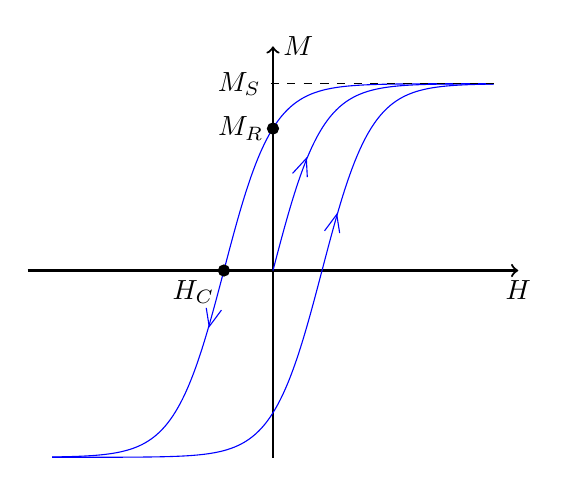
\begin{tikzpicture}
	\begin{axis}[
		xmin=-1.0,xmax=1.2,ymin=0,ymax=1.2,
  		axis lines=none,
  		samples=500]
  		
	 	\draw[thick,->] (axis cs:-1,0.5) -- (axis cs:1,0.5)node[anchor=north] {$H$};
	 	\draw[thick,->] (axis cs:0,-0.1) -- (axis cs:0,1.1)node[anchor=west] {$M$};
		\addplot[blue,domain=-0.9:0.9] {(1)/(1+exp(-10*x+2))};
		\addplot[blue,domain=-0.9:0.9] {(1)/(1+exp(-10*x-2))};									\addplot[blue,domain=0:0.9] {(1)/(1+exp(-10*x))};
		\addplot [only marks,mark=*] coordinates {(-0.2,0.5)};
		\addplot [only marks,mark=*] coordinates {(0,0.88)};
		\node[anchor=north east] at (axis cs:-0.2,0.5) {$H_{C}$};
	    \node[anchor=east] at (axis cs:0,0.88) {$M_{R}$};
    
		\draw[dashed] (axis cs:-0.01,1)node[anchor=east] {$M_{S}$} -- (axis cs:0.9,1);
		\draw[blue] (axis cs:0.08,0.76) -- (axis cs:0.136,0.8) -- (axis cs:0.14,0.75);
		\draw[blue] (axis cs:-0.21,0.394) -- (axis cs:-0.26,0.35) -- (axis cs:-0.272,0.4);
		\draw[blue] (axis cs:0.21,0.606) -- (axis cs:0.26,0.65) -- (axis cs:0.272,0.6);
		
    \end{axis}
  \end{tikzpicture}
\caption[Magnetic hysteresis cycle]{Magnetic hysteresis cycle. The magnetic material will retain a magnetic moment, $M_{R}$, even in the absence of an external field, which essentially creates a new permanent magnet. Only at a coercive field, $H_{C}$, the net magnetic moment of the material will return to zero.}%
\label{fig:magneticHysteresis}
\end{figure}
Key parameters of the hysteresis loop are the remanent magnetization or remanence $M_{R}$, which is the residual magnetization after the external field is removed and the coercivity $H_{C}$, which is the magnitude of the field that must be applied in the negative direction to bring the magnetization back to zero.\
%
\subsection{Magnetic materials and properties}\label{subsec:magneticMaterialsAndProperties}
Magnetic materials encompass a wide variety of materials and their macroscopic magnetic behaviour can be classified into ferro- or ferrimagnetic, paramagnetic and diamagnetic.\ They are grouped according to their magnetic dipole orientation and bulk magnetic susceptibility, which is schematically shown in Figure~\ref{fig:magneticMaterialProperty}.\ The different kinds of magnetism will be briefly discussed in the following subsections.\
\begin{figure}[htb]
        \centering
        \begin{subfigure}[b]{0.29\textwidth}
        \centering
                \includegraphics[width=\textwidth]{img/chapters/chapter_2_theory/ferromagnetism_crop.png}
                \caption{Ferromagnetism}
                \label{fig:ferromagnetism}
        \end{subfigure}
        \hfill
        \begin{subfigure}[b]{0.29\textwidth}
        \centering
                \includegraphics[width=\textwidth]{img/chapters/chapter_2_theory/ferrimagnetism_crop.png}
                \caption{Ferrimagnetism}
                \label{fig:ferrimagnetism}
        \end{subfigure}
        \hfill
        \begin{subfigure}[b]{0.29\textwidth}
        \centering
		        \includegraphics[width=\textwidth]{img/chapters/chapter_2_theory/paramagnetism_crop.png}			
                \caption{Paramagnetism}
                \label{fig:paramagnetism}
        \end{subfigure}
        \caption[Overview and comparison of the different types of magnetism]{Overview and comparison of the different types of magnetism. The magnetic dipole orientation defines the magnetic type.}
        \label{fig:magneticMaterialProperty}
\end{figure}
%
\subsubsection{Ferromagnetic and ferrimagnetic materials}\label{subsec:ferromagneticAndFerrimagneticMaterials}
Ferromagnetic and ferrimagnetic materials are the ones normally thought of as magnetic, because these materials are the only ones that can retain a significant magnetization and become magnets.\ The magnetic moments interact strongly with an applied magnetic field and their orientation remains stable even after removal of the external field.\ Thus, ferromagnetic materials exhibit a large and positive magnetic susceptibility ($\chi \gg 0$).\\
Different classes of spontaneous magnetization have been identified when there are multiple magnetic moments, whose magnitude and arrangement can be different and arranged anti-parallel.\ In the case of ferromagnetism, all magnetic moments are aligned parallel to one another, which results in a strong positive interaction between neighbouring moments, whereas in the ferrimagnetic case some magnetic moments are anti-aligned resulting in a weaker net magnetization $\mathbf{M}$, as shown in Figure~\ref{fig:ferromagnetism} and Figure~\ref{fig:ferrimagnetism}~\cite{Chikazumi1964}.\\
The ease with which the different domains can change their direction differs widely between the different ferro- and ferrimagnetic materials.\ However, this wide variety of magnetic materials can be rather sharply divided into two groups.\ If a small applied field suffices to produce saturation, the material is said to be magnetically soft (e.g. iron, iron-silicon alloys or low-carbon steels).\ Other materials, which require a very large field to saturate are called magnetically hard (e.g. neodymium magnet, Alnico or Strontium ferrite)~\cite{Cullity2011,Chikazumi1964,Krishnan2016}.\ The difference can be best seen in their hysteresis loops as depicted in Figure~\ref{fig:magneticSoftMagneticHard}.\
\begin{figure}[htb]
        \centering
        \begin{subfigure}[b]{0.48\textwidth}
                \begin{tikzpicture}[scale=1.0]
                \begin{axis}[
		  		axis lines=none,
  				samples=500]
  		
			 		\draw[thick,->] (axis cs:-0.8,0.5) -- (axis cs:0.8,0.5)node[anchor=north east] {$H$};
		 			\draw[thick,->] (axis cs:0,-0.1) -- (axis cs:0,1.1)node[anchor=north east] {$M$};
					\addplot[blue,domain=-0.7:0.7] {(1)/(1+exp(-30*x+1))};
					\addplot[blue,domain=-0.7:0.7] {(1)/(1+exp(-30*x-1))};
					\addplot[blue,domain=0:0.7] {(1)/(1+exp(-30*x))};
					
					\draw[blue] (axis cs: -0.066,0.42) -- (axis cs: -0.049,0.39) -- (axis cs: -0.026,0.42);
					\draw[blue] (axis cs: 0.066,0.58) -- (axis cs: 0.049,0.61) -- (axis cs: 0.026,0.58);
					\draw[blue] (axis cs: 0.015,0.713) -- (axis cs: 0.035,0.75) -- (axis cs: 0.045,0.71);
			    \end{axis}
            	
				\end{tikzpicture}
                \caption{Soft magnetic}
                \label{fig:magneticSoft}
        \end{subfigure}
        \hfill
        \begin{subfigure}[b]{0.48\textwidth}
                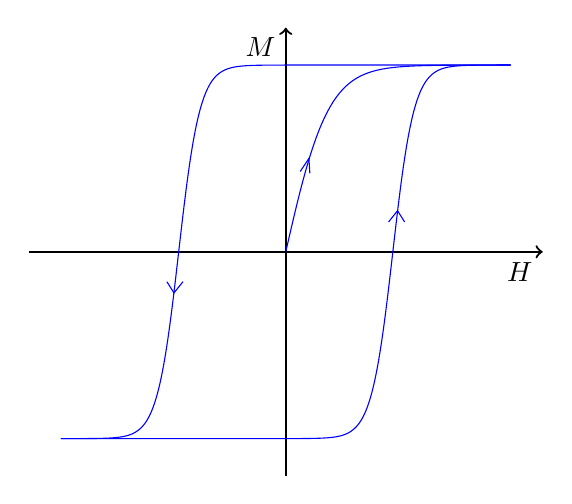
\begin{tikzpicture}[scale=1.0]
                \begin{axis}[
		  		axis lines=none,
		  		samples=500]
  		
	 				\draw[thick,->] (axis cs:-0.8,0.5) -- (axis cs:0.8,0.5)node[anchor=north east] {$H$};
				 	\draw[thick,->] (axis cs:0,-0.1) -- (axis cs:0,1.1)node[anchor=north east] {$M$};
					\addplot[blue,domain=-0.7:0.7] {(1)/(1+exp(-30*x+10))};
					\addplot[blue,domain=-0.7:0.7] {(1)/(1+exp(-30*x-10))};
					\addplot[blue,domain=0:0.7] {(1)/(1+exp(-15*x))};
					
					\draw[blue] (axis cs: 0.045,0.715) -- (axis cs: 0.072,0.75) -- (axis cs: 0.075,0.71);
					\draw[blue] (axis cs: 0.32,0.58) -- (axis cs: 0.348,0.61) -- (axis cs: 0.37,0.58);
					\draw[blue] (axis cs: -0.32,0.42) -- (axis cs: -0.348,0.39) -- (axis cs: -0.37,0.42);
					
				\end{axis}
				
				\end{tikzpicture}
                \caption{Hard magnetic}
                \label{fig:magneticHard}
        \end{subfigure}
        \caption[Hysteresis loops for soft and hard magnetic materials]{Hysteresis loop for ferromagnetic material. (a) A soft magnetic behaviour and (b) a hard magnetic behaviour.}
        \label{fig:magneticSoftMagneticHard}
\end{figure}
%
\subsubsection{Paramagnetic materials}\label{subsec:paramagneticMaterials}
Like ferromagnetic species, paramagnetic materials contain magnetic moments which align when exposed to a magnetic field such that they form a weak net magnetic moment, which means their magnetic susceptibility is small and positive ($\chi > 0$).\\
However, unlike ferromagnetic materials, they do not exhibit magnetic remanence upon removal of the field as the individual magnetic moments of the different domains become randomized due to thermal agitation and do not interact with each other.\ Thus, paramagnetic materials are only magnetized in the presence of an externally applied field, and once the field is removed the magnetization is lost~\cite{Coey2010,Chikazumi1964}.\
%
\subsubsection{Superparamagnetic materials}\label{subsec:superparamagneticMaterials}
Even if its name suggests a subtype of paramagnetism, superparamagnetism is actually a special form of magnetism with characteristics from both ferromagnetism and paramagnetism.\ When the length scale of the magnetic material becomes smaller than a critical size ($10-20$ nm), the ferro- or paramagnetic grains can essentially be considered as individual magnetic domains and their magnetization is a single magnetic moment~\cite{Ohandley2000}.\ At this scale, the available thermal energy becomes of the same order as the magnetic energy, causing the magnetic moment to immediately align randomly in space, after the magnetic field has been removed.\ Therefore, the coercivity and remanence is substantially equal to zero and thus, no hysteresis can be observed~\cite{Brown1963,McNab1968,Rosensweig2013}.\\
This behaviour can be described by the N\'{e}el relaxation time which describes the time needed for a magnetic moment to change its orientation~\cite{Neel1949}:\
\begin{equation}
	\tau = \tau_{0}\cdot \text{exp}\big(\frac{\Lambda V}{k_{B}T}\big)
	\label{eqn:neelRelaxationTime}
\end{equation}
where the different parameters $\Lambda$, $V$, $k_{B}$ and $T$ are the magnetic anisotropy energy density, grain volume, Boltzmann constant and the temperature, respectively.\ The height of the energy barrier is given by $\Lambda V$ and $k_{B}T$ is the thermal energy.\ $\tau_{0}$ is the material characteristic time scale, normally in the order of $0.1-1$ nanoseconds.\\
The magnetic susceptibility of these commercially available beads is typically in the range of $0.01-1.5$~\cite{Zborowski2015,Fonnum2005,Haefeli2005,Wise2015}.\
%
\subsubsection{Diamagnetic materials}\label{subsec:dieamagneticMaterials}
Diamagnetic materials exhibit a net magnetization which is opposite to the direction of the externally applied magnetic field and thus, are repelled by the applied magnetic field.\ That means, diamagnetic materials have a small negative magnetic susceptibility ($-1<\chi<0$)~\cite{Cullity2011}.\ Examples for diamagnetic materials are gold, copper or water~\cite{Krishnan2016}.\\
The opposed magnetic moment of diamagnetic substances is generally a very weak effect and loses its opposing magnetization after removal of the applied magnetic field.\
%
\section{Theory of magnetophoresis}\label{sec:theoryOfMagnetophoresis}
Magnetophoresis is the combination of fluid dynamics (Section~\ref{sec:fluidMotionInMicrofluidicSystems}) and magnetism (Section~\ref{sec:magnetism}).\\
A magnetic particle that is in suspension in a liquid and is being exposed to a magnetic field, experiences a set of forces.\ However, the magnetic force and the Stokes drag force are the most dominant forces relevant to this thesis.\ Other forces such as, gravity, buoyancy and also Saffman forces can be neglected for the microscopic particles used because of their small size ($1$ $\mu$m $-2.8$ $\mu$m) compared to the channel dimensions ($0.4\times3$ mm) and the time-scales involved~\cite{McCloskey2000,Wirix-Speetjens2005,Saffman1965}.\ Thus, Newton's second law of motion can be written as~\cite{Kreyszig2006}:\
\begin{equation}
	V_{p}\rho_{p} \frac{\partial \mathbf{u}_{p}}{\partial t} = \mathbf{F}_{m}+\mathbf{F}_{d}
	\label{eqn:equationOfMotion}
\end{equation}
where $\mathbf{F}_{m}$ and $\mathbf{F}_{d}$ describe the two dominant forces, the magnetic force and the Stokes drag, respectively.\ The two parameters $V_{p}$ and $\rho_{p}$ describe the particle volume and its density.\ Thus, the product of the two is the mass of the particle.\\
The magnetic force on a magnetized object $\mathbf{F}_{m}$ can be expressed in multiple ways~\cite{Plonus1978}:\
\begin{eqnarray}
	\mathbf{F}_{m}	&=& V_{p} \chi_{p}(\mathbf{H}\cdot \nabla)\mathbf{B} 
	\label{eqn:magneticForceMagneticField} \\
	 						&=& \frac{V_{p} \chi_{p}}{\mu_{0}}\Bigl( \mathbf{B}\cdot \nabla \Bigr)\mathbf{B} 
	\label{eqn:magneticForceMagneticFlux}	
\end{eqnarray}
where $V_{p}$ and $\chi_{p}$ are the volume and the effective susceptibility of the particle, respectively.\ Equation~\ref{eqn:magneticForceMagneticFlux} is most commonly used in the literature and will also be used throughout this thesis.\\
If the particle is suspended in a viscous fluid, Equation~\ref{eqn:magneticForceMagneticFlux} needs to be slightly modified since the susceptibility of the surrounding medium should be taken into account~\cite{Zborowski2011}:\
\begin{equation}
	\mathbf{F}_{m} = \Delta \chi V_{p} \left(\frac{\nabla |\mathbf{B}|^{2}}{2\mu_{0}}\right)
	\label{eqn:magneticForceFluid}
\end{equation}
where $\Delta \chi = \chi_{p}-\chi_{f}$ describes the difference in relative magnetic susceptibility between the magnetic particle ($\chi_{p}$) and the surrounding medium ($\chi_{f}$).\\
It is important to note here, that Equation~\ref{eqn:magneticForceMagneticField}-\ref{eqn:magneticForceFluid} assume a constant magnetic field across the volume of the particle and the magnetic media to be linearly polarizable, for which the magnetic susceptibility $\chi_{p}$ is independent of the applied magnetic field.\ In general, this is a valid assumption for all materials in a sufficiently weak field.\\
In the case of micrometre sized spherical particles at low Reynolds number, Stokes regime is found to be applicable (see Section~\ref{subsec:particleLadenFlowInMicrofluidicSystems}) and the Stokes drag force in Equation~\ref{eqn:equationOfMotion} can be assumed as~\cite{Happel2012}:\
\begin{equation}
	\mathbf{F_{d}} = -6\pi\eta_{f} r_{p} \Delta u
	\label{eqn:dragForceOnParticle}
\end{equation}
where $r_{p}$ is the particle's radius, $\eta_{f}$ the viscosity of the medium the particle is suspended in, and $\Delta u = u_{f}-u_{p}$ is the relative velocity between the particle and the fluid.\\
For micro-sized particles, a terminal velocity is reached in a matter of microseconds, in which case it is appropriate to assume~\cite{Abbasov1999}:
\begin{equation}
	\mathbf{F}_{m} = -\mathbf{F}_{d}
	\label{eqn:equationOfMotionSimplified}
\end{equation}
From this simplified equation of motion (Equation~\ref{eqn:equationOfMotionSimplified}) and the two equations, Equation~\ref{eqn:magneticForceFluid} and Equation~\ref{eqn:dragForceOnParticle}, one obtains the magnetically induced terminal velocity of the particle:\
\begin{equation}
	\mathbf{u}_{p} = \underbrace{\frac{\Delta\chi_{p} V_{p}}{6\pi\eta r_{p}}}_{\begin{smallmatrix}{\text{Material}}\\{\text{properties}}\end{smallmatrix}} \cdot \underbrace{\left(\frac{\nabla |\mathbf{B}|^{2}}{2\mu_{0}}\right)}_{\begin{smallmatrix}{\text{Magnetic field}}\\{\text{properties}}\end{smallmatrix}}
	\label{eqn:terminalVelocity}
\end{equation}
An interesting interpretation of the expression given in Equation~\ref{eqn:terminalVelocity}, is that it depends on a purely material related term and a field related term; it is a product of particle and suspending viscous medium properties and the applied magnetic field properties.\ The two factors of this product can be defined as the magnetophoretic mobility of the particle $\nu_{p}$ and the magnetophoretic driving force $S$, given by:\
\begin{eqnarray}
		\nu_{p} &=& \frac{\Delta \chi V_{p}}{6\pi\eta r_{p}} \label{eqn:magnetophoreticMobility} \\
		S &=& \frac{\nabla |\mathbf{B}|^{2}}{2\mu_{0}} \label{eqn:magnetophoreticDrivingForce}
\end{eqnarray}
The magnetically induced terminal velocity (Equation~\ref{eqn:terminalVelocity}) can be used to model the trajectory of a single magnetic particle in a magnetic field with the help of the Lagrangian particle tracking scheme, which will be discussed in the next section.\
%
\subsection{Lagrangian particle tracking}\label{subsec:lagrangianParticleTracking}
The Lagrangian tracking scheme is based on Newton's equation of motion (Equation~\ref{eqn:equationOfMotion}) and maps the positions of a single particle at discrete time steps.\ The mathematical expression for the tracking scheme can be given by:\
\begin{equation}
	\mathbf{x}(t+\delta t) = \mathbf{x}(t)+\mathbf{u}_{p}\delta t
	\label{eqn:lagrangianEquation}
\end{equation}
in which $\mathbf{x}(t)$ is the location vector of the particle at time $t$, $\mathbf{u}_{p}$ is the instantaneous particle velocity vector (see Equation~\ref{eqn:terminalVelocity}) and $\delta t$ is an incremental time interval, small enough so that the particle velocity vector $\mathbf{u}_{p}$ is essentially constant during the finite time step $\delta t$.\ In solving the equation of motion (Equation~\ref{eqn:equationOfMotionSimplified}) in a Lagrangian approach, the trajectory of single magnetic particles can be simulated.\ Thereby, time step, $\delta t$, needs to meet the Courant-Friedrich-Lewy (CFL) condition to guarantee accuracy and computational stability of the particle trajectory solution~\cite{Courant1967}:\
\begin{equation}
	\frac{\mathbf{u}_{p}^{i}\delta t}{\omega} \leq 1
	\label{eqn:courantFriedrichsLewy} 
\end{equation}
where $\mathbf{u}_{p}^{i}$, $\delta t$ and $\omega$ are the velocity vector of the $i^{\text{th}}$ particle, the time marching step and the grid size of the simulated magnetic field, respectively.\ The simulation of the magnetic field, using FEM, is the subject of the next section.\
%
\section{Mathematical formulation of finite element equations for magnetostatic problems}
\label{sec:mathematicalFormulationOfFiniteElementEquations}
All macroscopic electromagnetic phenomena are governed by a set of equations, known as the Maxwell's equations.\ For the magnetostatic problem, where the magnetic field is time-invariant and the electric field can be neglected, the magnetic field must satisfy the following differential equations~\cite{Maxwell1873}:\
\begin{eqnarray}
	\mathbf{\nabla} \times \mathbf{H} &=& \mathbf{J} \label{eqn:ampereLaw} \\
	\mathbf{\nabla} \cdot \mathbf{B} &=& 0 \label{eqn:gaussLaw} \\
	\mathbf{B} &=& \mu_{0}\mu_{r}\mathbf{H} \label{eqn:simpleLaw}
\end{eqnarray}
where $\mathbf{H}$, $\mathbf{B}$ and $\mathbf{J}$ are the magnetic field intensity, the magnetic flux density and the current density, respectively.\ The magnetic flux density can be expressed in terms of its vector potential $\mathbf{\Phi}$~\cite{Maxwell1873}:\
\begin{equation}
	\mathbf{B} = \mathbf{\nabla} \times \mathbf{\Phi}
	\label{eqn:magneticFluxVectorPotential}
\end{equation}
Substituting Equation~\ref{eqn:magneticFluxVectorPotential} into Equation~\ref{eqn:ampereLaw} with the aid of Equation~\ref{eqn:simpleLaw} yields the second-order differential equation~\cite{Maxwell1873}:\
\begin{equation}
	\nabla \times \left(\frac{1}{\mu_{0}\mu_{r}}\nabla \times \mathbf{\Phi} \right) = \mathbf{J}
	\label{eqn:vectorPotential}
\end{equation}
Assuming the magnetic permeability is isotropic and independent of the magnetic field, Equation~\ref{eqn:vectorPotential} can be written as Poisson's equation~\cite{Maxwell1873}:\
\begin{equation}
	\mathbf{\nabla}^{2} \mathbf{\Phi} = \Delta \mathbf{\Phi} = \mu_{0}\mu_{r}\mathbf{J} \text{ in } \Omega
	\label{eqn:vectorPotentialPoissonEquation}
\end{equation}
where $\Delta$ is the Laplace operator and the vector potential $\mathbf{\Phi}$ needs to be a real function in the problem domain $\Omega$ with boundary $\partial \Omega$.\ This boundary value problem can be further formulated as a variational expression~\cite{ansys2010}:\
\begin{equation}
	E(\mathbf{\Phi}) = \frac{1}{2}\int_{\Omega}\left(\frac{\nabla\mathbf{\Phi} \cdot \nabla\mathbf{\Phi}}{\mu_{0}\mu_{r}}-\mathbf{\Phi} \cdot \mathbf{J}\right)d\Omega
	\label{eqn:energyFunctional}
\end{equation}
However, the vector potential $\mathbf{\Phi}$ in Equation~\ref{eqn:energyFunctional} is formulated as a continuous function, which FEM cannot deal with.\ Therefore, the continuous problem in Equation~\ref{eqn:energyFunctional} is broken into a discrete physical representation consisting of a finite number of regions or finite elements.\\
The discretization of the domain $\Omega$ is normally the first step in FEM.\ One of the most commonly used approaches for two-dimensional (2D) and three-dimensional (3D) problems, is to divide the domain into a mesh of triangles or tetrahedra, respectively.\ These basic building blocks, triangle or tetrahedral, are called elements and are depicted in Figure~\ref{fig:typicalFiniteElements}.\
\begin{figure}[htb]
	\centering
	\begin{subfigure}[b]{0.48\textwidth}
		\centering
		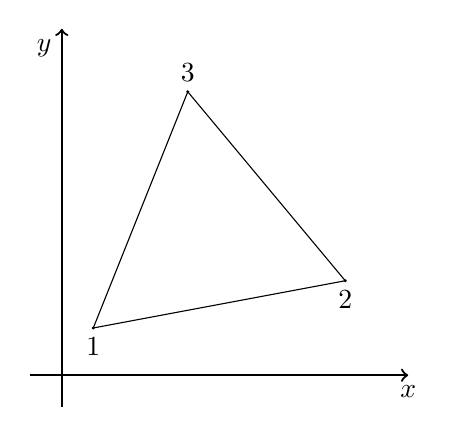
\begin{tikzpicture}[scale=0.4]
		\draw[thick,->] (-1,0)  -- (11,0) node[anchor=north] {$x$};
	  	\draw[thick,->] (0,-1) -- (0,11) node[anchor=north east] {$y$};
  
  		\coordinate[label=below:$1$] 	(p1) at (1,1.5);
		\coordinate[label=below:$2$] 	(p2) at (9,3);
		\coordinate[label=above:$3$] 	(p3) at (4,9);
	
		\fill (p1) circle (1.5pt);
		\fill (p2) circle (1.5pt);
		\fill (p3) circle (1.5pt);
  
  		\draw (p1) -- (p2) -- (p3) -- cycle;
		\end{tikzpicture}
		\caption{Triangular}
		\label{fig:triangularElement}
	\end{subfigure}
  	\hfill
	\begin{subfigure}[b]{0.48\textwidth}
		\centering
  		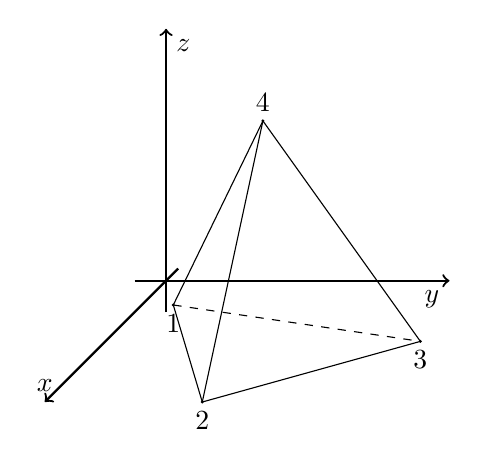
\begin{tikzpicture}[scale=0.4]
		\draw[thick,->] (-1,0,0) -- (9,0,0) node[thick,anchor=north east]{$y$};
		\draw[thick,->] (0,-1,0) -- (0,8,0) node[thick,anchor=north west]{$z$};
		\draw[thick,->] (0,0,-1) -- (0,0,10) node[thick,anchor=south]{$x$};
	
		\coordinate[label=below:$1$] 	(p1) at (1,0,2);
		\coordinate[label=below:$2$] 	(p2) at (5,0,10);
		\coordinate[label=below:$3$] 	(p3) at (10,0,5);
		\coordinate[label=above:$4$] 	(p4) at (5,7,5);
	
		\fill (p1) circle (1.5pt);
		\fill (p2) circle (1.5pt);
		\fill (p3) circle (1.5pt);
		\fill (p4) circle (1.5pt);
  
		\draw[solid] 	(p1) -- (p2);
		\draw[dashed] (p1) -- (p3);
		\draw[solid] 	(p2) -- (p3);
		\draw[solid] 	(p1) -- (p4);
		\draw[solid] 	(p2) -- (p4);
		\draw[solid] 	(p3) -- (p4);
	\end{tikzpicture} 
	\caption{Tetrahedral}
	\label{fig:tetrahedralElement}
\end{subfigure}
\caption[Typical finite elements: triangular element and tetrahedral element]{Typical finite elements: (a) triangular element and (b) tetrahedral element.}
  \label{fig:typicalFiniteElements}
\end{figure}
In each element the unknown function $\mathbf{\Phi}$ is represented by a trial function $\tilde{\mathbf{\Phi}}$, where the desired field in each element is approximated with a $2\textsuperscript{nd}$ order quadratic polynomial~\cite{ansys2010}:\
\begin{equation}
	\tilde{\mathbf{\Phi}}(x,y,z) = a_{0}+a_{1}x+a_{2}y+a_{3}z+a_{4}xy+a_{5}yz+a_{6}xz+a_{7}x^{2}+a_{8}y^{2}+a_{9}z^{2}
	\label{eqn:basisFunction}
\end{equation}
The parameters $a_{i}$ are unknown values, which need to be found.\ In order to obtain these values, field quantities are calculated for 10 points of each element, shown in Figure~\ref{fig:finiteElementMethodPoints}.\
\begin{figure}[htb]
\centering
  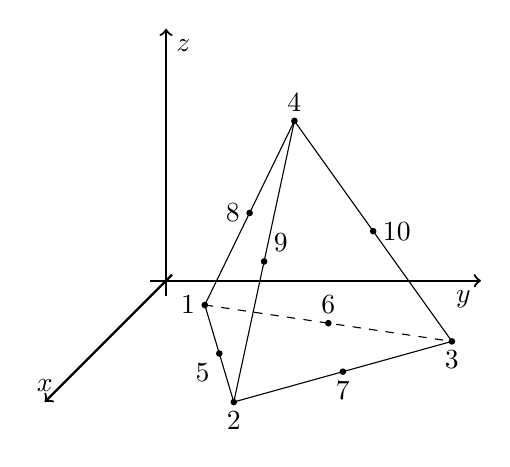
\begin{tikzpicture}[scale=0.4]
  \draw[thick,->] (-1.5,0,0) -- (9,0,0) node[thick,anchor=north east]{$y$};
  \draw[thick,->] (-1.0,-0.5,0) -- (-1.0,8,0) node[thick,anchor=north west]{$z$};
	\draw[thick,->] (-1.0,0,-0.5) -- (-1.0,0,10) node[thick,anchor=south]{$x$};
	
	\coordinate[label=left:$1$] 	(p1) at (1,0,2);
	\coordinate[label=below:$2$] 	(p2) at (5,0,10);
	\coordinate[label=below:$3$] 	(p3) at (10,0,5);
	\coordinate[label=above:$4$] 	(p4) at (5,7,5);
	\coordinate[label=below left:$5$] 	(p5) at (3,0,6);				
	\coordinate[label=above:$6$] 	(p6) at (5.5,0,3.5);
	\coordinate[label=below:$7$] 	(p7) at (7.5,0,7.5);
	\coordinate[label=left:$8$] 	(p8) at (3,3.5,3.5);
	\coordinate[label=above right:$9$] 	(p9) at (5,3.5,7.5);
	\coordinate[label=right:$10$] 	(p10) at (7.5,3.5,5);
		
	\fill (p1) circle (3pt);
	\fill (p2) circle (3pt);
	\fill (p3) circle (3pt);
	\fill (p4) circle (3pt);
	\fill (p5) circle (3pt);
	\fill (p6) circle (3pt);
	\fill (p7) circle (3pt);
	\fill (p8) circle (3pt);
	\fill (p9) circle (3pt);
	\fill (p10) circle (3pt);
  
  \draw[solid] 	(p1) -- (p2);
  \draw[dashed] (p1) -- (p3);
  \draw[solid] 	(p2) -- (p3);
  \draw[solid] 	(p1) -- (p4);
  \draw[solid] 	(p2) -- (p4);
  \draw[solid] 	(p3) -- (p4);
  
	\end{tikzpicture} 
  \caption[Interpolation points on a single element in FEM]{Points for which the magnetic vector potential will be calculated in the FEM. Field quantities inside the tetrahedral are calculated using a $2\textsuperscript{nd}$ order quadratic interpolation scheme.}
  \label{fig:finiteElementMethodPoints}
\end{figure}
The solution to these points, which solves Equation~\ref{eqn:vectorPotentialPoissonEquation}, can then be obtained by minimizing the energy functional (Equation~\ref{eqn:energyFunctional}) with respect to the values $a_{i}$ and subject to the given boundary conditions and user defined initial conditions.\ This calculation is done at each node in every tetrahedral which results in a large, sparse matrix equation, which can be solved using standard matrix solution techniques.\ Proof can be found in~\cite{Mikhlin1964}.\
%
\subsection{Error estimation of the finite element method}
\label{sec:errorEstimationOfTheFiniteelementMethod}
Even though FEM has evolved into one of the most widely used techniques for finding approximate solutions to differential equations it suffers from one major problem.\ The very act of subdividing the domain $\Omega$ provides the opportunity for \emph{discretization errors}.\ First, discretization errors occur because the \emph{finite} element model is, by definition, incapable of reproducing every one of the \emph{infinite} solution patterns that the problem domain can assume.\ Second, the construction of these subsets of the domain is not a trivial task, since the mesh must satisfy nearly contradictory requirements: it must conform to the shape of the object or simulation domain; its elements must be neither too large nor too numerous; it may have to grade from small to large elements over a relatively short distance; and it must be composed of elements that are of the right shapes and sizes.\ Such a mesh is known as a \textit{regular mesh} and is achieved by keeping the aspect ratio of its elements below a positive constant $\vartheta$~\cite{Cheng2012}:\
\begin{equation}
	\theta = \frac{\varrho_{out}}{\varrho_{in}} \leq \vartheta
	\label{eqn:meshRegularity}
\end{equation}
where $\varrho_{out}$ and $\varrho_{in}$ are the outer and inner diameter of the element (triangle or tetrahedral), respectively.\ If $\vartheta$ is small, normally $\vartheta\leq 5$, the mesh quality is considered to be sufficient.\ The literature demonstrates that the accuracy of finite element solutions on triangular meshes degrades as angles are allowed to approach $180^{\circ}$~\cite{Cheng2012}.\ Figure~\ref{fig:meshShape} visually illustrates these effects.\ The three triangulations are each using $200$ triangles to render a paraboloid.\ It can be seen that the mesh of Figure~\ref{fig:small}, where the mesh is composed by long thin triangles with no angle greater than $90^{\circ}$, only performs slightly worse than the isotropic triangulation in Figure~\ref{fig:normal}.\ However, when the angles approach $180^{\circ}$ as shown in Figure~\ref{fig:large}, the solution gets more distorted.\
\begin{figure}[htb!]
\centering
	\begin{subfigure}[b]{\textwidth}
		\centering
		\begin{minipage}[t]{0.48\textwidth}
		\includegraphics[width=\textwidth]{img/chapters/chapter_2_theory/normalAngleMesh.eps}
		\end{minipage}
		\begin{minipage}[t]{0.48\textwidth}
		\includegraphics[width=\textwidth]{img/chapters/chapter_2_theory/normalAngleResult.eps}
		\end{minipage}
		\caption{Isotropic triangles}
        \label{fig:normal}
	\end{subfigure}
	%%%%%%%%%%%
	\begin{subfigure}[b]{\textwidth}
		\centering
		\begin{minipage}[t]{0.48\textwidth}
		\includegraphics[width=\textwidth]{img/chapters/chapter_2_theory/smallAngleMesh.eps}
		\end{minipage}
		\begin{minipage}[t]{0.48\textwidth}
		\includegraphics[width=\textwidth]{img/chapters/chapter_2_theory/smallAngleResult.eps}
		\end{minipage}
		\caption{Sharp angle triangles}
        \label{fig:small}
	\end{subfigure}
	%%%%%%%%%%%
	\begin{subfigure}[b]{\textwidth}
		\centering
		\begin{minipage}[t]{0.48\textwidth}
		\includegraphics[width=\textwidth]{img/chapters/chapter_2_theory/largeAngleMesh.eps}
		\end{minipage}
		\begin{minipage}[t]{0.48\textwidth}
		\includegraphics[width=\textwidth]{img/chapters/chapter_2_theory/largeAngleResult.eps}
		\end{minipage}
		\caption{Obtuse angle triangles}
        \label{fig:large}
	\end{subfigure}
	\caption[Illustration how large angles in element negatively effect FEM results]{Visual illustration of how large angles negatively effect the result of the FEM solution. The left hand side of each subfigure shows the mesh used to render the 2D parabolic function (right hand side). Each mesh has exactly 200 triangles where a) contains isotropic triangles, b) has sharp angle triangles and c) is made of obtuse angle triangles.}
    \label{fig:meshShape}
\end{figure}
%
\subsubsection{Adaptive mesh refinement algorithm}\label{subsubsec:adaptiveMeshRefinement}
The difference between the exact solution $\mathbf{\Phi}$ and the nummerical approximation $\tilde{\mathbf{\Phi}}$ is the discretization error~\cite{Ainsworth2011}:\
\begin{equation}
	\epsilon = \|\mathbf{\Phi} - \tilde{\mathbf{\Phi}}\|_{\star}
	\label{eqn:discretizationError} 
\end{equation}
The discretization error can be given in any given norm, which is indicated by the asterisk, but always depends on the number of elements in the mesh; i.e. the finer the mesh, the smaller the discretization error.\ Adaptive mesh refinement is an approach to minimise the discretization error by locally refining the mesh where errors are particularly high.\ This process is then repeated until an end criteria is reached, e.g. the required accuracy is met or the maximum number of iteration steps is reached.\ Figure~\ref{fig:boxFlowDiagramAdaptiveMeshAlgorithm} schematically illustrates the adaptive mesh refinement algorithm.\
\begin{figure}[htb]
	\centering
	\includegraphics[width=0.6\textwidth]{img/chapters/chapter_2_theory/boxFlowDiagramAdaptiveMeshingCycle.pdf}
	\caption[Box flow diagram of an adaptive mesh refinement algorithm]{Box flow diagram of an adaptive mesh refinement algorithm used in various FEM programs.}
	\label{fig:boxFlowDiagramAdaptiveMeshAlgorithm}
\end{figure}
Multiple adaptive mesh refinement algorithms are described in the literature~\cite{Ainsworth2011,Verfurth2013}; e.g. more mesh points are placed in areas where the gradient of the solution is highest or the mesh is refined according to the change in the derivative at the element boundaries~\cite{Babuska1981,Zienkiewicz1987}.\ Another approach, which will be used in this thesis, is using the residuals in the elements~\cite{Zienkiewicz1983}:\
\begin{equation}
	\varepsilon_{e} = \Delta \tilde{\mathbf{\Phi}} - \mathbf{J}
\end{equation}
The parameter $\varepsilon_{e}$ indicates how well the original equations are locally satisfied by the approximate solution.\ The generated mesh is required to meet acceptable energy error estimate~\cite{ansys2010}:\
\begin{equation}
	\xi_{e} = \frac{|\varepsilon_{e}|}{E(\tilde{\mathbf{\Phi}})}
	\label{eqn:localPercentEnergyErrorEstimate}
\end{equation}
where $\xi_{e}$ is the local energy error in element $e$ and $E(\tilde{\mathbf{\Phi}})$ describes the total energy in the discrete system, which for the FEM approximate solution can be formulated as the following (also see Equation~\ref{eqn:energyFunctional})~\cite{ansys2010}:\
\begin{equation}
	E(\tilde{\mathbf{\Phi}}) = \frac{1}{2}\int_{\Omega}\left(\frac{\nabla \tilde{\mathbf{\Phi}} \cdot \nabla \tilde{\mathbf{\Phi}}}{\mu_{0}\mu_{r}}+\tilde{\mathbf{\Phi}} \cdot \mathbf{J} \right)d\Omega
	\label{eqn:totalEnergy}
\end{equation}
The $\xi_{e}$ values act as an energy error estimate criteria and are used for adaptive mesh refinement.\ Summing the local errors in each element and dividing the sum by the total energy leads to a global percentage error energy~\cite{ansys2010}:\
\begin{equation}
	\xi = \frac{\sum_{e=1}^{n}|\varepsilon_{e}|}{E(\tilde{\mathbf{\Phi}})} \times 100
	\label{eqn:globalPercentEnergyErrorEstimate}
\end{equation}
Equation~\ref{eqn:globalPercentEnergyErrorEstimate} is used as a stopping criteria in order to terminate the refinement process.\
%
\section{Statistical data analysis}\label{s:statisticalInference}
Part of the analysis in this thesis includes statistical testing.\ The basis and the concepts of the analysis are introduced here, but will be used later in the thesis.\\
In general, all processes are affected by \textit{chance} to a certain degree.\ Thus, every single measurement will be affected by small variances because of experimental errors.\ These random effects also occur in engineering problems because fabrication and other procedures are prone to small variations.\ The magnetic particles are not immune to these random variations due to small uncontrollable differences in their composition or shape.\\
A common aim of statistical analysis is to produce information (e.g. mean or variance) about a certain population.\ A \textit{population} is any well defined collection or set of values.\ This sense of the term population differs from the sense in which most social scientists use the term, as social scientists tend to view collections of people or objects as defining a population.\\
Since testing an entire population can be very lengthy, one often makes inferences (generalizations) where a subset of the population (statistical data sample) is chosen to represent the population.\ This process is also known as \textit{statistical interference}~\cite{Peck2015}.\ Selecting a statistical sample has its pitfalls, but the challenges of sampling will not be discussed here.\ There is a large body of work on sampling in the literature which the interested reader can consult~\cite{Peck2015,Box1978,Rosenbaum1985,Silverman1986}.\\
The sample mean (Equation~\ref{eqn:sampleMean}) and the sample variance (Equation~\ref{eqn:sampleVariance}) for a sample with $N$ observations can be expressed as~\cite{Peck2015}:\
\begin{eqnarray}
	\bar{x} &=& \frac{1}{N}\sum_{j=1}^{N}x_{j} = \frac{1}{N}(x_{1}+x_{2}+ \cdots + x_{N})
	\label{eqn:sampleMean} \\
	s^{2} &=& \frac{1}{N-1}\sum_{j=1}^{N}(x_{j}-\bar{x})^{2} = \frac{1}{n-1}\left[(x_{1}-\bar{x})^{2}+\cdots+(x_{N}-\bar{x})^{2}\right]
	\label{eqn:sampleVariance}
\end{eqnarray}
The variables $x_{j}$ are considered independent random variables, each corresponding to one randomly selected observation.\ Note that the sample mean (Equation~\ref{eqn:sampleMean}) and sample variance (Equation~\ref{eqn:sampleVariance}) are estimates of the population mean and population variance.\ With increasing sample size $N$ the difference between the sample and the population moments can be neglected.\ In this work, the statistical samples are the different particle types.\ Every observation of a single particle is assumed to be an independent random variable, which means the occurrence of one observation does not affect the probability of occurrence of another observation~\cite{Hogg1995}.\
%
\subsection{Significance testing}\label{subsec:significanceTesting}
Once sample data has been gathered through an observational study or quantitative research, statistical inference allows evidence in favour of a claim or hypothesis about a population statistic from which the sample has been drawn to be tested.\ The methods of inference used to support or reject claims on a sample data are known as significance tests.\\
Every significance test begins with a \textit{null hypothesis} $H_{0}$.\ The null hypothesis represents a theory that has been assumed, either because it is believed to be true or because it is to be used as a basis for arguments.\\
The \textit{alternative hypothesis} $H_{a}$ is a statement of what a statistical hypothesis test aims to establish.\\
The conclusion once the test has been carried out is always given in terms of the null hypothesis.\ Either $H_{0}$ is accepted (which does not necessarily mean that the null hypothesis is true) except for a small error probability $\alpha$, called the \textit{acceptance level}, or $H_{0}$ is rejected in favour of $H_{a}$.\ Hence $\alpha$ is the probability of rejecting a hypothesis although it is true (Type I error).\ The choice of $\alpha$ is up to the person who performs the test.\ Common values are $\alpha = 5\%$ or $\alpha = 1\%$.\\
In deciding which test is appropriate to use, it is important to consider the type of variables, i.e. whether the variables are categorical, ordinal or interval and what distribution the variables have~\cite{Kreyszig2006,Mohr1990}.\ In this study, the mean values of different magnetic particle samples will be tested using a \textit{one-way analysis of variance} (ANOVA) with an acceptance level $\alpha = 5\%$.\ The one-way ANOVA is used to determine whether there are any statistically significant differences between the means of three or more independent groups.\ Specifically, it tests the null hypothesis $H_{0}$:\
\begin{equation}
	H_{0}: \mu_{1} = \mu_{2} = \cdots = \mu_{n}
\end{equation}
where the different $\mu_{i}$ are the different means of the separate groups and the index $n$ the number of groups.\ If, however, the one-way ANOVA returns a statistically significant result, the alternative hypothesis $H_{a}$ is accepted, i.e. there are at least two group means that are significantly different from each other.\ At this point, it is important to state that the one-way ANOVA cannot tell which specific groups are significantly different from each other, only that there are at least two.\ To determine which specific groups differ from each other, a post-hoc test needs to be performed.\\
Whenever the one-way ANOVA is used the following assumptions are made:\
\begin{itemize}
	\item The sample means $\bar{x}$ in each group are normally distributed.\ A normal distribution can usually be assumed for samples where the number of observations is large ($N\geq 30$) due to the central limit theorem~\cite{Kreyszig2006,Israel1992}.\
	\item There is homogeneity of variances, meaning the variances in each group are equal.\
	\item Independence of observations, which is already assumed when using Equation~\ref{eqn:sampleMean} and Equation~\ref{eqn:sampleVariance}.\
\end{itemize}
In this work, the ANOVA test will be used to compare the susceptibility values at different magnetic field strengths of two groups of magnetic beads.\ The two groups use different measurement approaches to determine the susceptibility of the bead population.\